\documentclass[10pt,letterpaper]{article}
\usepackage[latin1]{inputenc}
\usepackage[left=1in,right=1in,top=1in,bottom=1in]{geometry} 
\usepackage{amsmath}
\usepackage{amsfonts}
\usepackage{amssymb}
\usepackage{pagecolor}
\usepackage{tikz}
\usetikzlibrary{automata,positioning,decorations.pathreplacing}

\begin{document}
\pagecolor{white}
Game of Life 

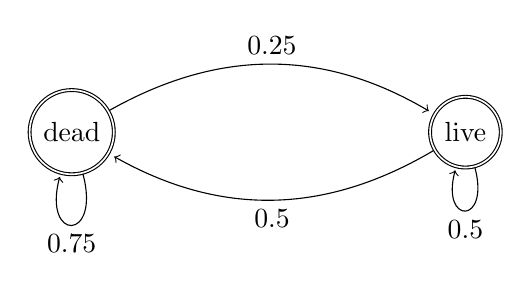
\begin{tikzpicture}[shorten >=2pt,node distance=5cm,on grid,auto] 
\node[state, accepting] (q_0) {dead};
\node[state, accepting] (q_4) [right=of q_0] {live};    

\path[->]
(q_0) edge [bend left, above] node {0.25} (q_4)  
(q_4) edge [bend left, below] node {0.5} (q_0)  

(q_0) edge [loop below] node {0.75} (q_0)
(q_4) edge [loop below] node {0.5} (q_4)
; %end path 
\end{tikzpicture}




(A1) Instant birth, gradual death, no recovery.  

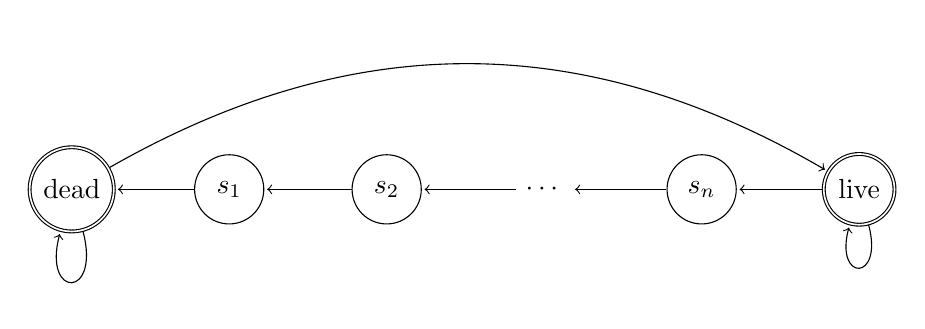
\begin{tikzpicture}[shorten >=1pt,node distance=2cm,on grid,auto] 
\node[state, accepting] (q_0) {dead};
\node[state] (q_1) [right=of q_0] {$s_1$};
\node[state] (q_2) [right=of q_1] {$s_2$};
\node        (q_dots) [right=of q_2] {$\cdots$}; 
\node[state] (q_3) [right=of q_dots] {$s_{n}$};
\node[state, accepting] (q_4) [right=of q_3] {live};    

\path[->]
(q_0) edge [bend left, above] node {} (q_4)  
(q_1) edge node {} (q_0)  
(q_0) edge [loop below] node {} (q_0)
(q_2) edge node {} (q_1) 
(q_3) edge  node {} (q_dots) 
(q_dots) edge node{} (q_2)
(q_4) edge node {} (q_3) 
(q_4) edge [loop below] node {} (q_4)
; %end path 
\end{tikzpicture}   \\

(A2) Instant birth, gradual death, stay sick, no recovery.  

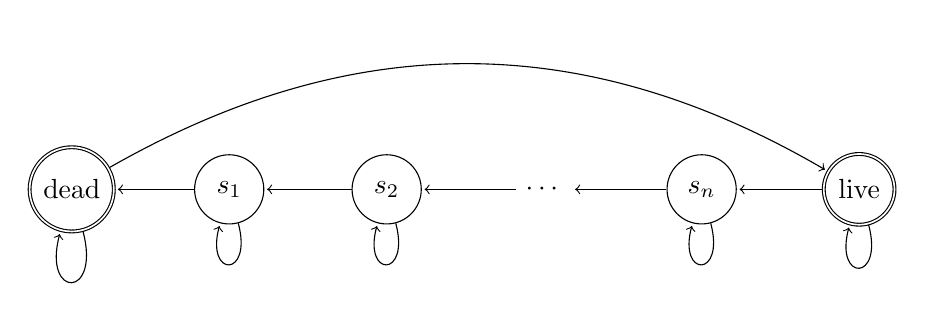
\begin{tikzpicture}[shorten >=1pt,node distance=2cm,on grid,auto] 
\node[state, accepting] (q_0) {dead};
\node[state] (q_1) [right=of q_0] {$s_1$};
\node[state] (q_2) [right=of q_1] {$s_2$};
\node        (q_dots) [right=of q_2] {$\cdots$}; 
\node[state] (q_3) [right=of q_dots] {$s_{n}$};
\node[state, accepting] (q_4) [right=of q_3] {live};    

\path[->]
(q_0) edge [bend left, above] node {} (q_4)  
(q_1) edge node {} (q_0)  
(q_0) edge [loop below] node {} (q_0)
(q_1) edge [loop below] node {} (q_1)
(q_2) edge [loop below] node {} (q_2)
(q_3) edge [loop below] node {} (q_3)
(q_2) edge node {} (q_1) 
(q_3) edge  node {} (q_dots) 
(q_dots) edge node{} (q_2)
(q_4) edge node {} (q_3) 
(q_4) edge [loop below] node {} (q_4)
; %end path 
\end{tikzpicture}   \\

(B1) Instant birth, gradual death, gradual recovery. 

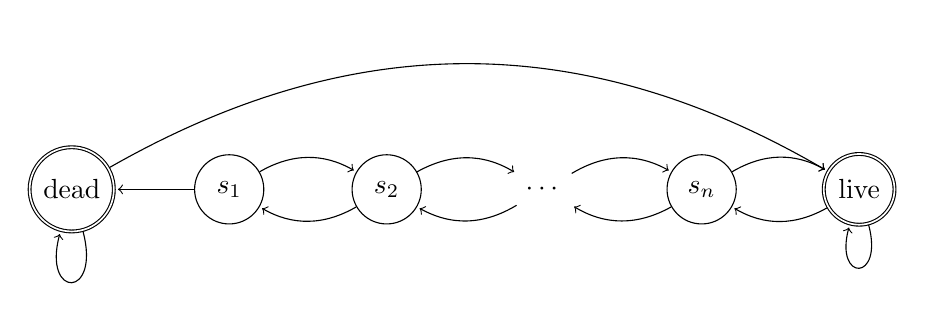
\begin{tikzpicture}[shorten >=1pt,node distance=2cm,on grid,auto] 
\node[state, accepting] (q_0) {dead};
\node[state] (q_1) [right=of q_0] {$s_1$};
\node[state] (q_2) [right=of q_1] {$s_2$};
\node        (q_dots) [right=of q_2] {$\cdots$}; 
\node[state] (q_3) [right=of q_dots] {$s_{n}$};
\node[state, accepting] (q_4) [right=of q_3] {live};    

\path[->]
(q_0) edge [loop below] node {} (q_0)
(q_4) edge [loop below] node {} (q_4)

(q_0) edge [bend left, above] node {} (q_4)  

(q_1) edge node {} (q_0)  

(q_2) edge [bend left, below] node {} (q_1) 
(q_1) edge [bend left, above] node {} (q_2) 

(q_dots) edge [bend left, below] node{} (q_2)
(q_2) edge [bend left, above] node{} (q_dots)


(q_3) edge [bend left, below] node {} (q_dots) 
(q_dots) edge [bend left, above] node {} (q_3)

(q_4) edge [bend left, below] node {} (q_3) 
(q_3) edge [bend left, above] node {} (q_4)
; %end path 
\end{tikzpicture}   \\


(B2) Instant birth, gradual death, gradual recovery. 

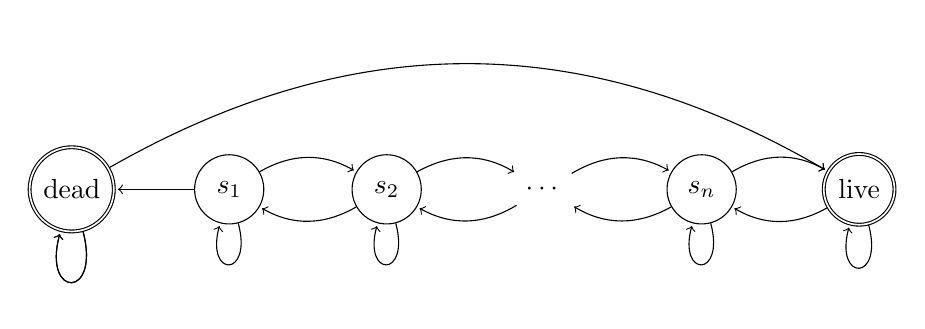
\begin{tikzpicture}[shorten >=1pt,node distance=2cm,on grid,auto] 
\node[state, accepting] (q_0) {dead};
\node[state] (q_1) [right=of q_0] {$s_1$};
\node[state] (q_2) [right=of q_1] {$s_2$};
\node        (q_dots) [right=of q_2] {$\cdots$}; 
\node[state] (q_3) [right=of q_dots] {$s_{n}$};
\node[state, accepting] (q_4) [right=of q_3] {live};    

\path[->]
(q_0) edge [loop below] node {} (q_0)
(q_4) edge [loop below] node {} (q_4)

(q_0) edge [bend left, above] node {} (q_4)  

(q_1) edge node {} (q_0)  

(q_2) edge [bend left, below] node {} (q_1) 
(q_1) edge [bend left, above] node {} (q_2) 

(q_dots) edge [bend left, below] node{} (q_2)
(q_2) edge [bend left, above] node{} (q_dots)


(q_3) edge [bend left, below] node {} (q_dots) 
(q_dots) edge [bend left, above] node {} (q_3)

(q_4) edge [bend left, below] node {} (q_3) 
(q_3) edge [bend left, above] node {} (q_4)

(q_0) edge [loop below] node {} (q_0)
(q_1) edge [loop below] node {} (q_1)
(q_2) edge [loop below] node {} (q_2)
(q_3) edge [loop below] node {} (q_3)
; %end path 
\end{tikzpicture}   \\

(C1) Instant birth, gradual death, instant death (Covid-19), gradual recovery. 

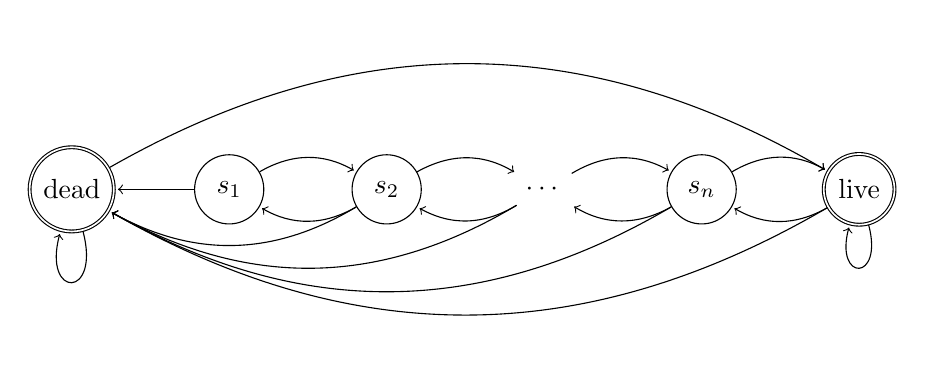
\begin{tikzpicture}[shorten >=1pt,node distance=2cm,on grid,auto] 
\node[state, accepting] (q_0) {dead};
\node[state] (q_1) [right=of q_0] {$s_1$};
\node[state] (q_2) [right=of q_1] {$s_2$};
\node        (q_dots) [right=of q_2] {$\cdots$}; 
\node[state] (q_3) [right=of q_dots] {$s_{n}$};
\node[state, accepting] (q_4) [right=of q_3] {live};    

\path[->]
(q_0) edge [loop below] node {} (q_0)
(q_4) edge [loop below] node {} (q_4)

(q_0) edge [bend left, above] node {} (q_4)  

(q_1) edge node {} (q_0)  

(q_2) edge [bend left, below] node {} (q_1) 
(q_1) edge [bend left, above] node {} (q_2) 
(q_2) edge [bend left, below] node {} (q_0) 

(q_dots) edge [bend left, below] node{} (q_2)
(q_2) edge [bend left, above] node{} (q_dots)
(q_dots) edge [bend left, below] node{} (q_0)

(q_3) edge [bend left, below] node {} (q_dots) 
(q_dots) edge [bend left, above] node {} (q_3)
(q_3) edge [bend left, below] node {} (q_0) 

(q_4) edge [bend left, below] node {} (q_3) 
(q_3) edge [bend left, above] node {} (q_4)
(q_4) edge [bend left, below] node {} (q_0) 
; %end path 
\end{tikzpicture}   \\

(C2) Instant birth, gradual death, instant death (Covid-19), gradual recovery. 

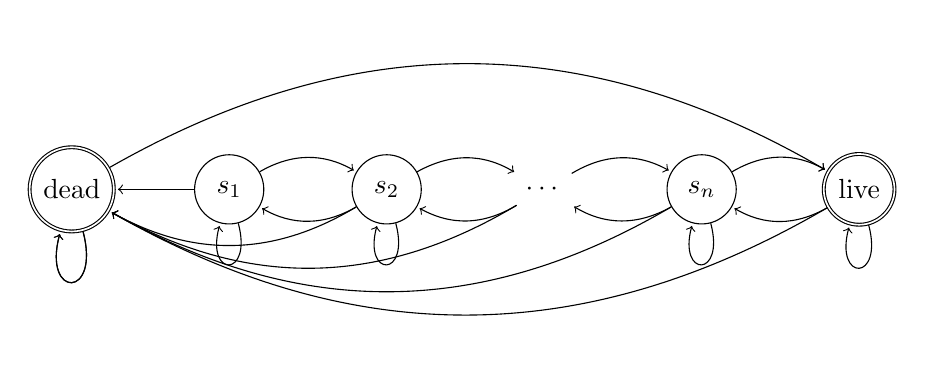
\begin{tikzpicture}[shorten >=1pt,node distance=2cm,on grid,auto] 
\node[state, accepting] (q_0) {dead};
\node[state] (q_1) [right=of q_0] {$s_1$};
\node[state] (q_2) [right=of q_1] {$s_2$};
\node        (q_dots) [right=of q_2] {$\cdots$}; 
\node[state] (q_3) [right=of q_dots] {$s_{n}$};
\node[state, accepting] (q_4) [right=of q_3] {live};    

\path[->]
(q_0) edge [loop below] node {} (q_0)
(q_4) edge [loop below] node {} (q_4)

(q_0) edge [bend left, above] node {} (q_4)  

(q_1) edge node {} (q_0)  

(q_2) edge [bend left, below] node {} (q_1) 
(q_1) edge [bend left, above] node {} (q_2) 
(q_2) edge [bend left, below] node {} (q_0) 

(q_dots) edge [bend left, below] node{} (q_2)
(q_2) edge [bend left, above] node{} (q_dots)
(q_dots) edge [bend left, below] node{} (q_0)

(q_3) edge [bend left, below] node {} (q_dots) 
(q_dots) edge [bend left, above] node {} (q_3)
(q_3) edge [bend left, below] node {} (q_0) 

(q_4) edge [bend left, below] node {} (q_3) 
(q_3) edge [bend left, above] node {} (q_4)
(q_4) edge [bend left, below] node {} (q_0) 

(q_0) edge [loop below] node {} (q_0)
(q_1) edge [loop below] node {} (q_1)
(q_2) edge [loop below] node {} (q_2)
(q_3) edge [loop below] node {} (q_3)
; %end path 
\end{tikzpicture}   \\

(D1) Gradual death, gradual recovery. 

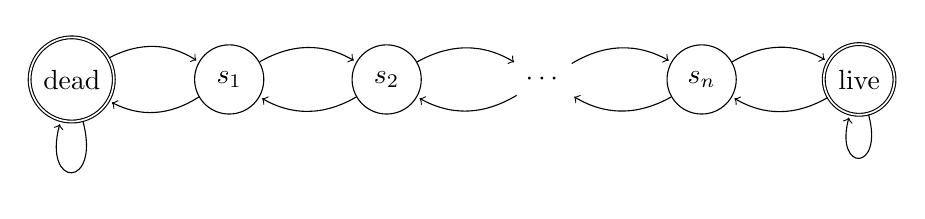
\begin{tikzpicture}[shorten >=1pt,node distance=2cm,on grid,auto] 
\node[state, accepting] (q_0) {dead};
\node[state] (q_1) [right=of q_0] {$s_1$};
\node[state] (q_2) [right=of q_1] {$s_2$};
\node        (q_dots) [right=of q_2] {$\cdots$}; 
\node[state] (q_3) [right=of q_dots] {$s_{n}$};
\node[state, accepting] (q_4) [right=of q_3] {live};    

\path[->]
(q_0) edge [loop below] node {} (q_0)
(q_4) edge [loop below] node {} (q_4)

(q_1) edge [bend left, below] node {} (q_0)  
(q_0) edge [bend left, above] node {} (q_1)  

(q_2) edge [bend left, below] node {} (q_1) 
(q_1) edge [bend left, above] node {} (q_2) 

(q_dots) edge [bend left, below] node{} (q_2)
(q_2) edge [bend left, above] node{} (q_dots)


(q_3) edge [bend left, below] node {} (q_dots) 
(q_dots) edge [bend left, above] node {} (q_3)

(q_4) edge [bend left, below] node {} (q_3) 
(q_3) edge [bend left, above] node {} (q_4)
; %end path 
\end{tikzpicture}   \\


(D2) Gradual death, gradual recovery. 

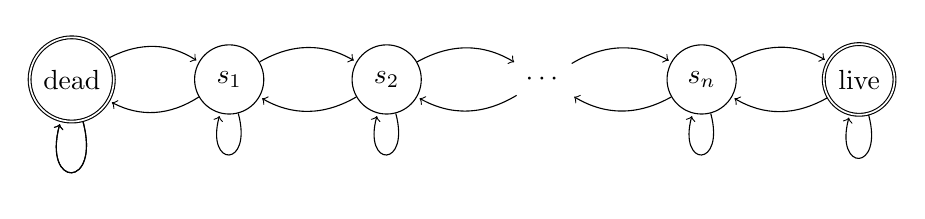
\begin{tikzpicture}[shorten >=1pt,node distance=2cm,on grid,auto] 
\node[state, accepting] (q_0) {dead};
\node[state] (q_1) [right=of q_0] {$s_1$};
\node[state] (q_2) [right=of q_1] {$s_2$};
\node        (q_dots) [right=of q_2] {$\cdots$}; 
\node[state] (q_3) [right=of q_dots] {$s_{n}$};
\node[state, accepting] (q_4) [right=of q_3] {live};    

\path[->]
(q_0) edge [loop below] node {} (q_0)
(q_4) edge [loop below] node {} (q_4)

(q_1) edge [bend left, below] node {} (q_0)  
(q_0) edge [bend left, above] node {} (q_1)  

(q_2) edge [bend left, below] node {} (q_1) 
(q_1) edge [bend left, above] node {} (q_2) 

(q_dots) edge [bend left, below] node{} (q_2)
(q_2) edge [bend left, above] node{} (q_dots)


(q_3) edge [bend left, below] node {} (q_dots) 
(q_dots) edge [bend left, above] node {} (q_3)

(q_4) edge [bend left, below] node {} (q_3) 
(q_3) edge [bend left, above] node {} (q_4)

(q_0) edge [loop below] node {} (q_0)
(q_1) edge [loop below] node {} (q_1)
(q_2) edge [loop below] node {} (q_2)
(q_3) edge [loop below] node {} (q_3)
; %end path 
\end{tikzpicture}   \\

(E1) Instant birth, any-level sick, gradual recovery. 

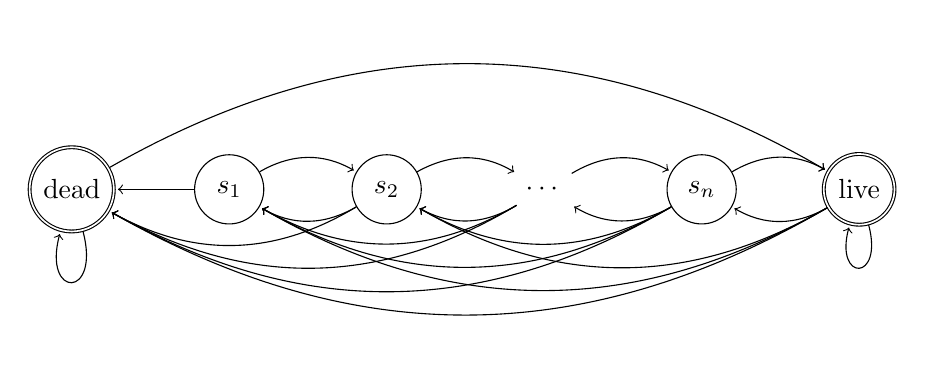
\begin{tikzpicture}[shorten >=1pt,node distance=2cm,on grid,auto] 
\node[state, accepting] (q_0) {dead};
\node[state] (q_1) [right=of q_0] {$s_1$};
\node[state] (q_2) [right=of q_1] {$s_2$};
\node        (q_dots) [right=of q_2] {$\cdots$}; 
\node[state] (q_3) [right=of q_dots] {$s_{n}$};
\node[state, accepting] (q_4) [right=of q_3] {live};    

\path[->]
(q_0) edge [loop below] node {} (q_0)
(q_4) edge [loop below] node {} (q_4)

(q_0) edge [bend left, above] node {} (q_4)  

(q_1) edge node {} (q_0)  

(q_2) edge [bend left, below] node {} (q_1) 
(q_1) edge [bend left, above] node {} (q_2) 
(q_2) edge [bend left, below] node {} (q_0) 

(q_dots) edge [bend left, below] node{} (q_0)
(q_dots) edge [bend left, below] node{} (q_1)
(q_dots) edge [bend left, below] node{} (q_2)
(q_2) edge [bend left, above] node{} (q_dots)

(q_3) edge [bend left, below] node {} (q_0) 
(q_3) edge [bend left, below] node {} (q_1)
(q_3) edge [bend left, below] node {} (q_2)  
(q_3) edge [bend left, below] node {} (q_dots) 
(q_dots) edge [bend left, above] node {} (q_3)


(q_4) edge [bend left, below] node {} (q_3) 
(q_4) edge [bend left, below] node {} (q_2) 
(q_4) edge [bend left, below] node {} (q_1) 
(q_4) edge [bend left, below] node {} (q_0) 
(q_3) edge [bend left, above] node {} (q_4)
; %end path 
\end{tikzpicture}   \\

(E2) Instant birth, any-level sick, gradual recovery. 

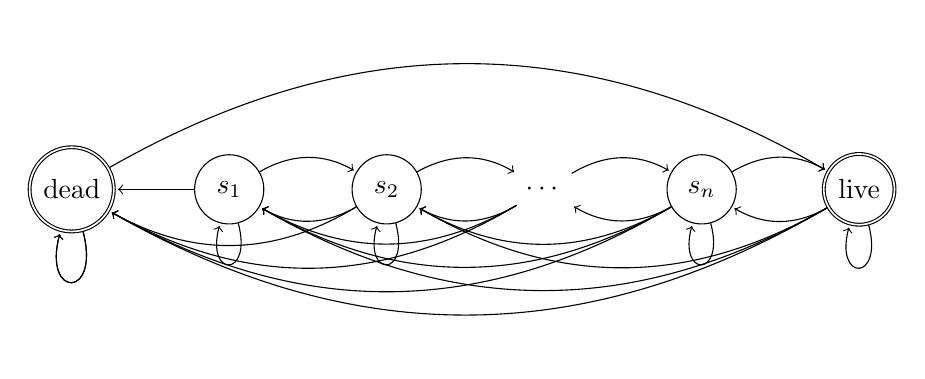
\begin{tikzpicture}[shorten >=1pt,node distance=2cm,on grid,auto] 
\node[state, accepting] (q_0) {dead};
\node[state] (q_1) [right=of q_0] {$s_1$};
\node[state] (q_2) [right=of q_1] {$s_2$};
\node        (q_dots) [right=of q_2] {$\cdots$}; 
\node[state] (q_3) [right=of q_dots] {$s_{n}$};
\node[state, accepting] (q_4) [right=of q_3] {live};    

\path[->]
(q_0) edge [loop below] node {} (q_0)
(q_4) edge [loop below] node {} (q_4)

(q_0) edge [bend left, above] node {} (q_4)  

(q_1) edge node {} (q_0)  

(q_2) edge [bend left, below] node {} (q_1) 
(q_1) edge [bend left, above] node {} (q_2) 
(q_2) edge [bend left, below] node {} (q_0) 

(q_dots) edge [bend left, below] node{} (q_0)
(q_dots) edge [bend left, below] node{} (q_1)
(q_dots) edge [bend left, below] node{} (q_2)
(q_2) edge [bend left, above] node{} (q_dots)

(q_3) edge [bend left, below] node {} (q_0) 
(q_3) edge [bend left, below] node {} (q_1)
(q_3) edge [bend left, below] node {} (q_2)  
(q_3) edge [bend left, below] node {} (q_dots) 
(q_dots) edge [bend left, above] node {} (q_3)


(q_4) edge [bend left, below] node {} (q_3) 
(q_4) edge [bend left, below] node {} (q_2) 
(q_4) edge [bend left, below] node {} (q_1) 
(q_4) edge [bend left, below] node {} (q_0) 
(q_3) edge [bend left, above] node {} (q_4)

(q_0) edge [loop below] node {} (q_0)
(q_1) edge [loop below] node {} (q_1)
(q_2) edge [loop below] node {} (q_2)
(q_3) edge [loop below] node {} (q_3)
; %end path 
\end{tikzpicture}   \\


\iffalse
\draw [decorate,decoration={brace,amplitude=10pt,mirror,raise=10pt},yshift=0pt]
(q_0.south west) -- (q_3.south east);
\fi
\end{document}